\chapter{System Description}\label{chap:sys_description}
The present chapter covers the system design including specific solutions that have been chosen for the realization of the SmartNotes application. The system concept, introduced in Chapter~\ref{chap:concept}, will become extended by describing certain elements of implementation and problems found during the development process. This should allow the reader have a deeper view into the SmartNotes application including functions that it offers and platform that it runs on.
\section{Google App Engine platform}\label{sec:gae}
Google App Engine seems to be an outstanding development platform. For all the reasons mentioned in~\ref{sec:gae_general}, it has been decided to be used as the main platform for SmartNotes before any other hosting services. Besides, GAE appears to be highly competitive in terms of cost calculations, which are described in Section~\ref{subsec:gae_calculations}. After registering the application with a unique name, it can be easily uploaded to Google and after a few seconds it is accessible to its users.

As stressed in Section~\ref{subsec:sync_scenarios}, synchronization scenarios use the client-server architecture. When running on GAE platform which is, as mentioned in~\ref{sec:gae_general}, a distributed vault-tolerant infrastructure where two subsequent request may be served by different machines located in separate data centres. Thus from the addressing scope the application can still be treated as a centralized server. In case the application requires state awareness it is the developer's role to make it so. Otherwise, the fact that the application is served from multiple machines is completely transparent from the functional point of view.

SmartNotes uses only some of the components supported by GAE and t he ones which make a part of SmartNotes application with relation with other third-party elements are presented in Figure~\ref{fig:smartnotes_components}. This is especially important as it presents all the application top level components together with marked interfaces between the particular functional blocks. This particular diagram strongly corresponds with the diagram from Figure~\ref{fig:ismartnotes_smartnotes}, which in a more general way presents the cooperation of SmartNotes and iSmartNotes with differentiated roles of the administrator and the user. 

The most complicated structure is the SmartNotes component, which is marked as an individual system. It does not require the iSmartNotes to realize its functionality. For this reason, the SmartNotes component could work with any kind of client application using the interface that the tool provides, or the interface of Mercurial HTTP chains of requests and responses that needed a back-end redesign to accommodate conditions set by GAE. The issues connected with the cooperation of Mercurial and GAE are the topic of Section~\ref{sec:hg_on_gae}. 

Furthermore, SmartNotes uses three additional interfaces which are used to interconnect the Google App Engine component with Mercurial adopted to run on GAE as well as separately, admin and user interfaces provided by SmartNotes. Each of the three components is connected in a different way. Whereas the webapp framework has a low Python overhead as mentioned in Section~\ref{subsec:webapp} and was chosen to serve the connection between the Mercurial and the Google App Engine componet, for performance reasons, it is Django which is the best choice when it comes to building nontrivial web-based functionality for reasons mentioned in Section~\ref{subsec:django}. The remaining two elements used by the GAE subsystem are the Google Account and the Datastore. The role of the first one has been presente in detail while discussing the iSmartNotes activation process in Section~\ref{subsec:ismartnotes_activation}. Some of the Datastore details will be covered in Section~\ref{sec:hg_on_gae}. 
\begin{figure}[ht]
\begin{center}
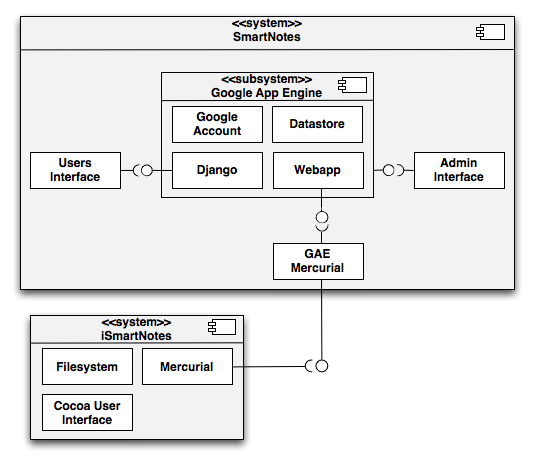
\includegraphics[scale=0.6]{charts/smartnotes_componets.png}
\caption{The components diagram of  the SmartNotes application with marked interfaces between the functional blocks.}
\label{fig:smartnotes_components}
\end{center}
\end{figure}

The second independent system is the iSmartNotes component, which remains independent until the user decides to activate it to use the synchronization feature. For this purpose, it requires a Mercurial server to interact with. The iSmartNotes, as presented in Figure~\ref{fig:smartnotes_components}, is build with three components. Firstly, the file system of the client's operating system which is the classical space where VCSs allocate their repositories. Secondly, Mercurial VCS which on the client site does not require any modifications. Finally, the Cocoa user interface whose presentation is provided in Section~\ref{sec:cocoa}.

\subsection{Financial calculations}\label{subsec:gae_calculations}
The role of this section is to introduce some general calculations that should give the reader a general experience of what resources will be used by the applications in connection with the billing rates set by Google. This values will be used to predict the size order of monthly cost for serving one million of SmartNotes users. This should should help to indicate the system elements that generate highest price resources usage what in effect lets to concentrate on the specific area optimization. 

Calculations below aim to predict theoretical monthly cost of running SmartNotes applications for one million active users with unit price list detailed in Table~\ref{tab:gae_cost}.Each of used resources will become briefly introduced with explanation of used assumptions to let the reader observe the proportion between outlined elements. The outcome of this considerations is illustrated in Figure~\ref{tab:gae_cost}.
\begin{table}[h]
\centering
\caption{Google App Engine billing rates on September 2009.}
\label{tab:gae_cost}
\begin{tabular}{|l|l|l|} \hline \hline
\textbf{Resource} & \textbf{Unit} & \textbf{Unit cost} \\ \hline \hline
Outgoing Bandwidth & Gigabytes & \$0.12 \\ \hline
Incoming Bandwidth & Gigabytes & \$0.10 \\ \hline
CPU Time & CPU hours & \$0.10 \\ \hline
Stored Data & Gigabytes per Day & \$0.005 \\ \hline
Recipients Emailed & Recipients & \$0.0001\\ \hline \hline
\end{tabular}
\end{table}


Resource usage to price calculations:
\begin{itemize}
\item{Outgoing Bandwidth. This value represents summarized amount of data send from the server to the users. This normally includes html, css, java script and graphic files as the standard web pages elements. In standard ca  }
\item{Incoming Bandwidth. }
\item{CPU Time. }
\item{Stored Data. }
\item{Mail. }
\end{itemize} 
This all together encloses in about \$314 without mailing and about \$410 for with mailing. Beside this the appilcation may use the free quota limits which are shown in Table~\ref{tab:gae_free} what should allow for reaching a rate of 5 million page views per month. This values could be compared to some popular hosting services like ... or ... that can offer same resources for respectively ... and ... for a service without mailing. Disregarding this difference it should be stressed that Google App Engine is not only a hosting service but also exposes for wide use Google infrastructure components that were mentioned in Section~\ref{sec:gae_general}.   
\begin{table}[h]
\centering
\caption{Google App Engine free quota limitations on September 2009.}
\label{tab:gae_cost}
\begin{tabular}{|l|l|} \hline \hline
\textbf{Resource} & \textbf{Daily Limit} \\ \hline \hline
Outgoing Bandwidth & 1 Gigabyte \\ \hline
Incoming Bandwidth & 1 Gigabyte \\ \hline
CPU Time & 6.5 CPU hours \\ \hline
Stored Data & 1 Gigabyte \\ \hline
Recipients Emailed & 2000 \\ \hline \hline
\end{tabular}
\end{table}


\begin{figure}[ht]
  \begin{center}
    \subfigure[\textbf{Without mailing service}.]{\label{fig:gae_cost_without_mail}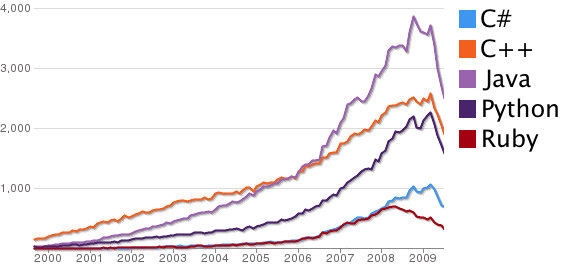
\includegraphics[scale=0.36]{img/Monthly_projects.png}}
    \subfigure[\textbf{With mailing service}.]{\label{fig:gae_cost_with_mail}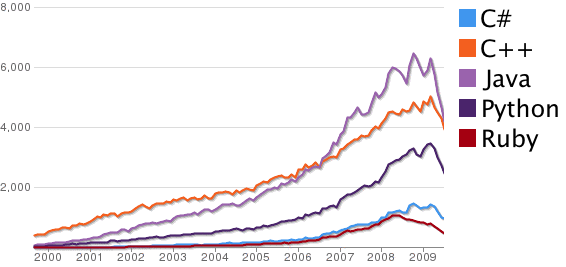
\includegraphics[scale=0.36]{img/Monthly_contributors.png}}
  \end{center}
  \caption{Simulated monthly cost division of resources expected to be used by one million of SmartNotes users.}
  \label{fig:gae_cost}
\end{figure}


\section{Mercurial on Google App Engine}\label{sec:hg_on_gae}
\section{Cocoa user interface}\label{sec:cocoa}